% *********************************************************************
% © 2026 Jeremy Sylvestre
%
% Permission is granted to copy, distribute and/or modify this document
% under the terms of the GNU Free Documentation License, Version 1.3 or
% any later version published by the Free Software Foundation; with no
% Invariant Sections, no Front-Cover Texts, and no Back-Cover Texts. A
% copy of the license is included in the appendix entitled “GNU Free
% Documentation License” that appears in the output document of this
% PreTeXt source code. All trademarks™ are the registered® marks of
% their respective owners.
%
% *********************************************************************
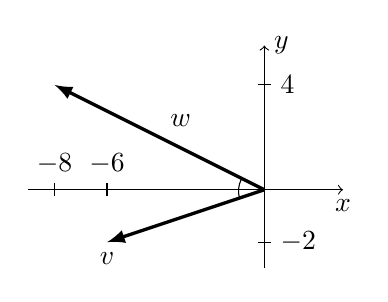
\begin{tikzpicture}[
	vector/.style={-latex,very thick},
	scale=0.333
]
	\draw[->] (-9,0) to (3,0) node[below] {$x$};
	\draw[->] (0,-3) to (0,5.5) node[right] {$y$};

	\draw[vector] (0,0) to node[at end,below] {$\uvec{v}$} (-6,-2);
	\draw[thin] (-6,-0.25) to (-6,0.25) node[above] {$-6$};
	\draw[thin] (-0.25,-2) to (0.25,-2) node[right] {$-2$};

	\draw[vector] (0,0) to node[above right] {$\uvec{w}$} (-8,4);
	\draw[thin] (-8,-0.25) to (-8,0.25) node[above] {$-8$};
	\draw[thin] (-0.25,4) to (0.25,4) node[right] {$4$};

	% angle arc
	\draw (0,0) ++(198.435:1cm) arc (195.435:153.435:1cm);

\end{tikzpicture}
